\documentclass[12pt]{article}
\input{/Users/circle/Documents/博一下/homework/setting.tex}
\setcounter{secnumdepth}{2}
\usepackage{autobreak}
\usepackage{amsmath}
\setlength{\parindent}{2em}
\graphicspath{{../}}
\ziju{0.1pt}

%pdf文件设置
\hypersetup{
	pdfauthor={袁磊祺},
	pdftitle={计算流体力学上机作业2}
}

\title{
		\vspace{-1in} 	
		\usefont{OT1}{bch}{b}{n}
		\normalfont \normalsize \textsc{\LARGE Peking University}\\[0.2cm] % Name of your university/college \\ [25pt]
		\horrule{0.5pt} \\[0.2cm]
		\huge \bfseries{计算流体力学上机作业2} \\[-0.2cm]
		\horrule{2pt} \\[0.2cm]
}
\author{
		\normalfont 								\normalsize
		College of Engineering \quad 2001111690  \quad 袁磊祺\\	\normalsize
        \today
}
\date{}

\begin{document}

%%%%%%%%%%%%%%%%%%%%%%%%%%%%%%%%%%%%%%%%%%%%%%
\captionsetup[figure]{name={图},labelsep=period}
\captionsetup[table]{name={表},labelsep=period}
\renewcommand\contentsname{目录}
\renewcommand\listfigurename{插图目录}
\renewcommand\listtablename{表格目录}
\renewcommand\refname{参考文献}
\renewcommand\indexname{索引}
\renewcommand\figurename{图}
\renewcommand\tablename{表}
\renewcommand\abstractname{摘\quad 要}
\renewcommand\partname{部分}
\renewcommand\appendixname{附录}
\def\equationautorefname{式}%
\def\footnoteautorefname{脚注}%
\def\itemautorefname{项}%
\def\figureautorefname{图}%
\def\tableautorefname{表}%
\def\partautorefname{篇}%
\def\appendixautorefname{附录}%
\def\chapterautorefname{章}%
\def\sectionautorefname{节}%
\def\subsectionautorefname{小小节}%
\def\subsubsectionautorefname{subsubsection}%
\def\paragraphautorefname{段落}%
\def\subparagraphautorefname{子段落}%
\def\FancyVerbLineautorefname{行}%
\def\theoremautorefname{定理}%
\crefname{figure}{图}{图}
\crefname{equation}{式}{式}
\crefname{table}{表}{表}
%%%%%%%%%%%%%%%%%%%%%%%%%%%%%%%%%%%%%%%%%%%

\maketitle


编写一维完全气体Euler方程组的WENO3,WENO5程序,撰写报告,包括问题和算法描述,输出结果及讨论,程序说明。


\begin{equation}
	\left\{\begin{array}{c}
		\left(\begin{array}{c}
			\rho   \\
			\rho u \\
			E
		\end{array}\right)_{t}+\left(\begin{array}{c}
				\rho u       \\
				\rho u^{2}+p \\
				u(E+p)
			\end{array}\right)_x=0, \\
		p=(\gamma-1)\left(E-\frac{1}{2} \rho u^{2}\right),\ \gamma=1.4.
	\end{array}\right.
\end{equation}

计算动图可点击 \href{https://www.bilibili.com/video/BV1cp4y1t7Bc}{https://www.bilibili.com/video/BV1cp4y1t7Bc} 查看。

代码可点击 \href{https://github.com/circlelq/Computational-Fluid-Dynamics/tree/main/code2}{https://github.com/circlelq/Computational-Fluid-Dynamics/tree/main/code2} 查看。


\section{1}

初始条件
\begin{equation}
	\boldsymbol{U}=\left\{\begin{array}{ll}
		(1,0,2.5)^{\mathrm{T}},      & x<0.3, \\
		(0.125,0,0.25)^{\mathrm{T}}, & x>0.3.
	\end{array}\right.
\end{equation}

计算区间为 $[0,1],$ 输出时刻 $t=0.2 .$

对于方程
\begin{equation}
	u_t + f_x = 0,
\end{equation}
使用Steger-Warming 通量分裂方法是根据特征值 $\lambda_{i}$ 来完成的,首先将特征值分解为正负部分:
\begin{equation}
	\lambda_{i}^{+}=\frac{1}{2}\left(\lambda_{i}+\left|\lambda_{i}\right|\right), \quad \lambda_{i}^{-}=\frac{1}{2}\left(\lambda_{i}-\left|\lambda_{i}\right|\right) .
\end{equation}
进而将矩阵 $A$ 分为正负两部分
\begin{equation}
	A=T^{-1} \Lambda T=T^{-1}\left(\Lambda^{+}+\Lambda^{-}\right) T=A^{+}+A^{-},
\end{equation}
其中 $\Lambda, \Lambda^{\pm}$ 是对角线上是特征值的对角矩阵。于是正负通量为
\begin{equation}
	f^{+}=A^{+} U, \quad f^{-}=A^{-} U.
\end{equation}


\subsection{WENO3}

例如 $r=2$ 时, 插值得到的可能 $f_{j+\frac{1}{2}}^{\pm}$ 为
\begin{equation}
	f_{j+\frac{1}{2}}^{+}=\left\{\begin{array}{l}
		-\frac{1}{2} f_{j-1}^{+}+\frac{3}{2} f_{j}^{+} \\
		\frac{1}{2} f_{j}^{+}+\frac{1}{2} f_{j+1}^{+},
	\end{array}, \quad f_{j+\frac{1}{2}}^{-}=\left\{\begin{array}{l}
		\frac{3}{2} f_{j+1}^{-}-\frac{1}{2} f_{j+2}^{-} \\
		\frac{1}{2} f_{j+1}^{-}+\frac{1}{2} f_{j}^{-}
	\end{array}\right.\right..
\end{equation}
相应的三阶WENO插值为
\begin{align}
	\hat{f}_{j+\frac{1}{2}}^{+} & =\omega_{1} \hat{f}_{j+\frac{1}{2}}^{(1),+}+\omega_{2} \hat{f}_{j+\frac{1}{2}}^{(2),+}                 ,                                                                            \\
	\omega_{i}                  & =\frac{\widetilde{\omega}_{i}}{\widetilde{\omega}_{1}+\widetilde{\omega}_{2}}, \quad \widetilde{\omega}_{i}=\frac{\gamma_{l}}{\left(\varepsilon+\beta_{i}\right)^{2}}, \quad i=1,2, \\
	\gamma_{1}                  & =\frac{1}{3}, \quad \gamma_{2}=\frac{2}{3},                                                                                                                                         \\
	\beta_{1}                   & =\left(f_{j}^{+}-f_{j-1}^{+}\right)^{2}, \quad \beta_{2}=\left(f_{j+1}^{+}-f_{j}^{+}\right)^{2},                                                                                    \\
	\hat{f}                     & =\hat{f}^+ + \hat{f}^-.
\end{align}
其中$\varepsilon = 1\times 10^{-6}$.

可以得到半离散格式
\begin{equation}
	\frac{\dif}{\dif t}u + \frac{1}{h}\left(\hat{f}_{j+\frac{1}{2}}-\hat{f}_{j-\frac{1}{2}}\right)=0.
\end{equation}
然后再用三阶TVD性质的RK时间差分格式
\begin{equation}
	\begin{aligned}
		{u}^{(1)} & ={u}^{n}+\Delta t L\left({u}^{n}\right)    ,                                             \\
		{u}^{(2)} & =\frac{3}{4} {u}^{n}+\frac{1}{4} {u}^{(1)}+\frac{1}{4} \Delta t L\left({u}^{(1)}\right), \\
		{u}^{n+1} & =\frac{1}{3} {u}^{n}+\frac{2}{3} {u}^{(2)}+\frac{2}{3} \Delta t L\left({u}^{(2)}\right).
	\end{aligned}
	\label{eq:11}
\end{equation}
其中$L$是空间离散算符。

如\cref{fig:2weno3} 所示,WENO3的计算结果比之前用LF等格式算的结果更接近理论解。


\begin{figure}[htp]
	\centering
	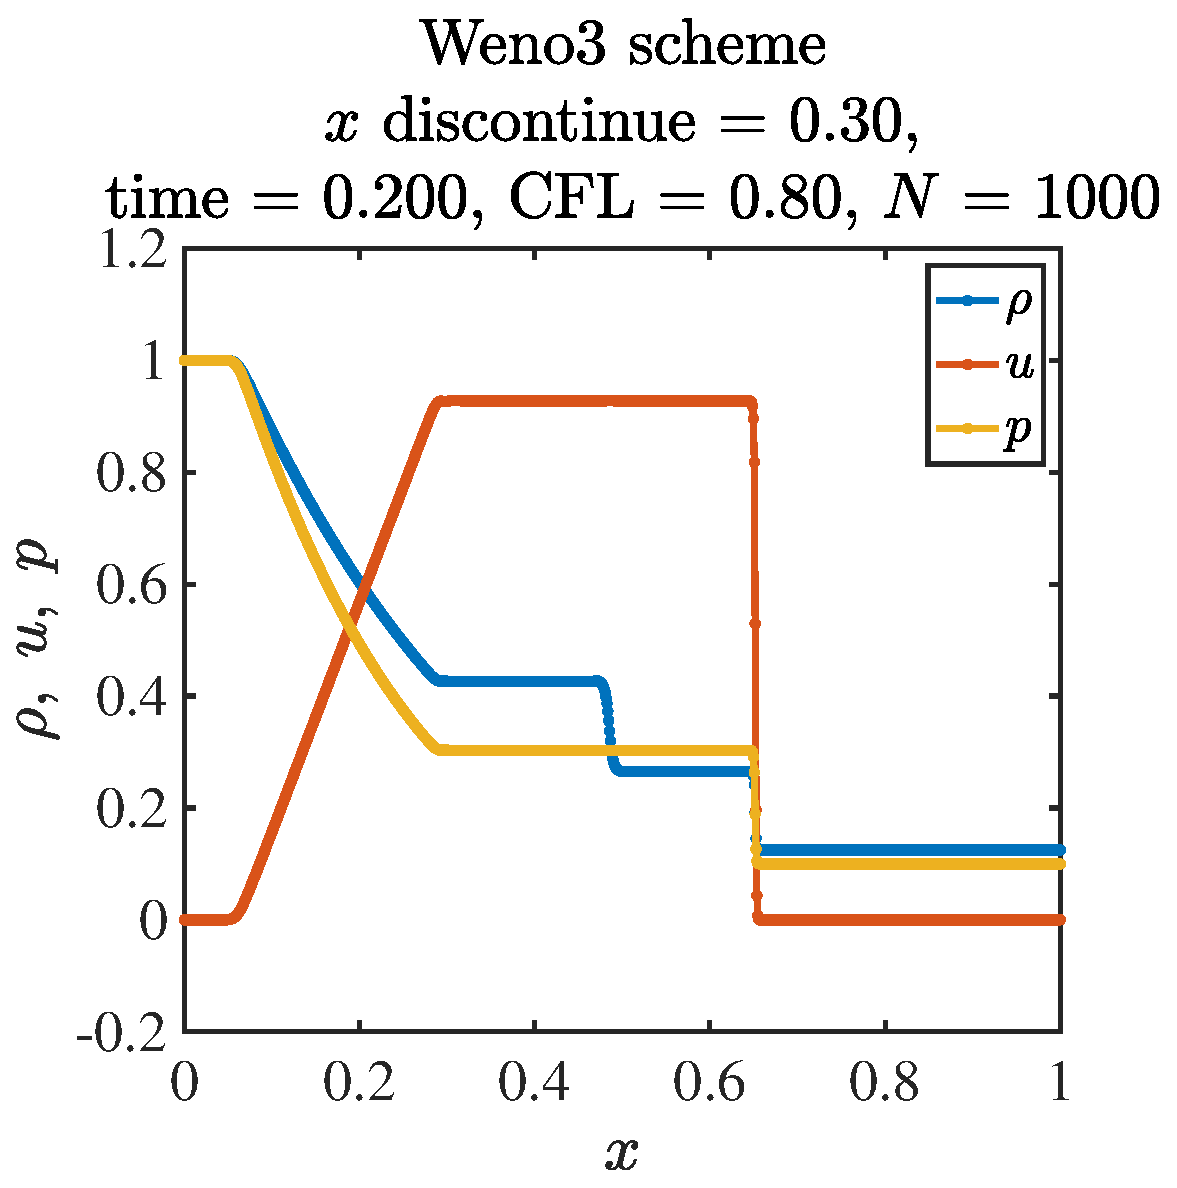
\includegraphics[width=10cm]{2weno3.eps}
	\caption{第二题WENO3格式。}
	\label{fig:2weno3}
\end{figure}

\subsection{WENO5}

WENO5采用的是使用三个长度为3的模版进行非线性组合
\begin{equation}
	u_{i+\frac{1}{2}}^{(1)}=\frac{3}{8} u_{i-2}-\frac{5}{4} u_{i-1}+\frac{15}{8} u_{i},
\end{equation}
\begin{equation}
	u_{i+\frac{1}{2}}^{(2)}=-\frac{1}{8} u_{i-1}+\frac{3}{4} u_{i}+\frac{3}{8} u_{i+1},
\end{equation}
\begin{equation}
	u_{i+\frac{1}{2}}^{(3)}=\frac{3}{8} u_{i}+\frac{3}{4} u_{i+1}-\frac{1}{8} u_{i+2},
\end{equation}
\begin{equation}
	u_{i+\frac{1}{2}}=w_{1} u_{i+\frac{1}{2}}^{(1)}+w_{2} u_{i+\frac{1}{2}}^{(2)}+w_{3} u_{i+\frac{1}{2}}^{(3)},
\end{equation}
\begin{equation}
	\begin{aligned}
		\beta_{1}=\frac{1}{3}\left(4 u_{i-2}^{2}-19 u_{i-2} u_{i-1}+25 u_{i-1}^{2}+11 u_{i-2} u_{i}-31 u_{i-1} u_{i}+10 u_{i}^{2}\right), \\
		\beta_{2}=\frac{1}{3}\left(4 u_{i-1}^{2}-13 u_{i-1} u_{i}+13 u_{i}^{2}+5 u_{i-1} u_{i+1}-13 u_{i} u_{i+1}+4 u_{i+1}^{2}\right),   \\
		\beta_{3}=\frac{1}{3}\left(10 u_{i}^{2}-31 u_{i} u_{i+1}+25 u_{i+1}^{2}+11 u_{i} u_{i+2}-19 u_{i+1} u_{i+2}+4 u_{i+2}^{2}\right).
	\end{aligned}
\end{equation}
\begin{equation}
	w_{j}=\frac{\tilde{w}_{j}}{\tilde{w}_{1}+\tilde{w}_{2}+\tilde{w}_{3}}, \quad \text { with } \quad \tilde{w}_{j}=\frac{\gamma_{j}}{\left(\varepsilon+\beta_{j}\right)^{2}},
\end{equation}
其中$\varepsilon = 1\times 10^{-6}$.
\begin{equation}
	\gamma_{1}=\frac{1}{16}, \quad \gamma_{2}=\frac{5}{8}, \quad \gamma_{3}=\frac{5}{16}.
\end{equation}
时间使用同样的离散方式\cref{eq:11}.如\cref{fig:2weno5} 所示,间断处的点比WENO3更少,更接近理论解。


\begin{figure}[htp]
	\centering
	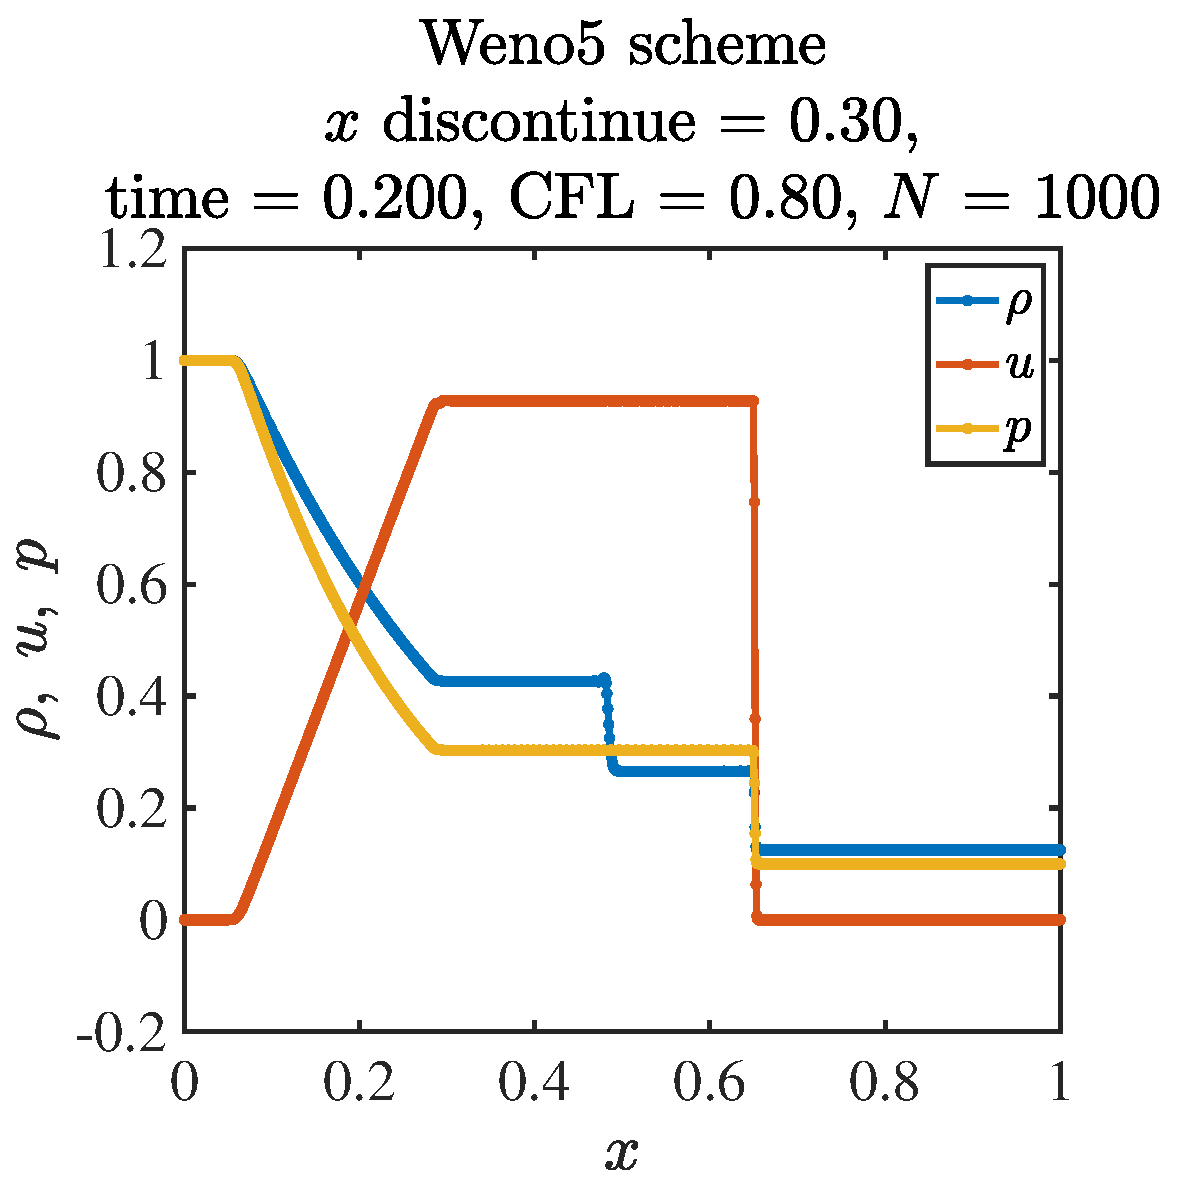
\includegraphics[width=10cm]{2weno5.eps}
	\caption{第二题WENO5格式。}
	\label{fig:2weno5}
\end{figure}




\section{2}

初 始 条 件
\begin{equation}
	(\rho, u, p)(x, 0)=\left\{\begin{array}{ll}
		(3.857143,2.629369,10.33333), & x<-4,     \\
		(1+0.2 \sin (5 x), 0,1),      & x \geq-4.
	\end{array}\right.
\end{equation}
计算区间为 $[-5,5]$, 其中在 $x=\pm 5$ 边界处 $\partial_{x} \rho=\partial_{x} u=\partial_{x} p=0 .$ 输出时刻 为 $t=1.8$.

如\cref{fig:4weno3,fig:4weno5} 所示,分别为WENO3和WNENO5的计算结果。可以发现接近激波的地方密度$\rho$震荡较剧烈,而且WENO5的震荡更明显,但是离激波较远的地方比较稳定。


\begin{figure}[htp]
	\centering
	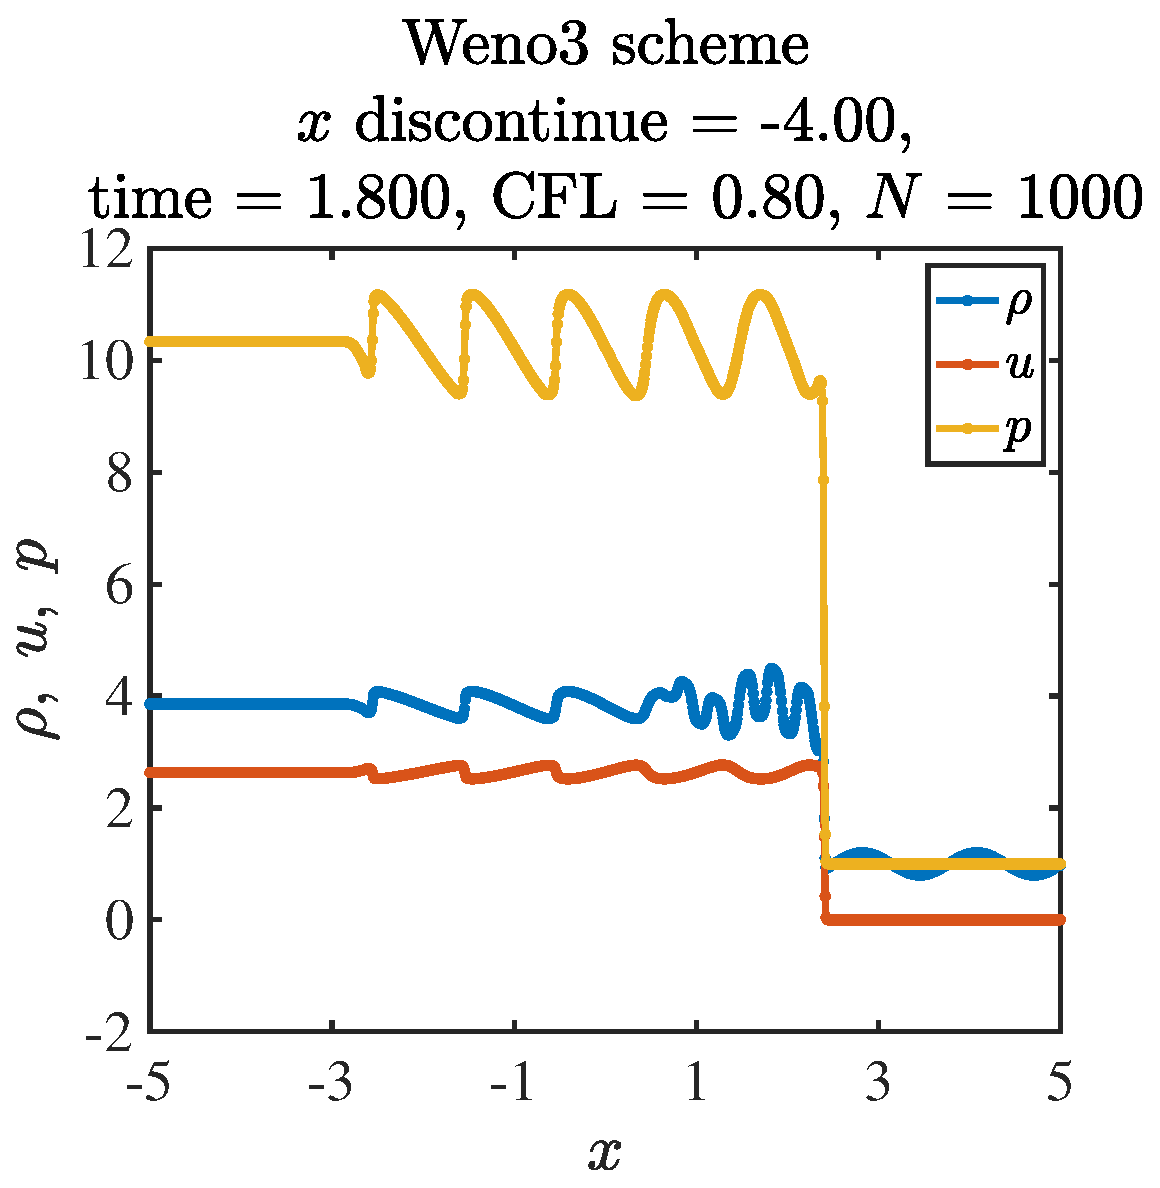
\includegraphics[width=10cm]{4weno3.eps}
	\caption{第四题WENO3格式。}
	\label{fig:4weno3}
\end{figure}

\begin{figure}[htp]
	\centering
	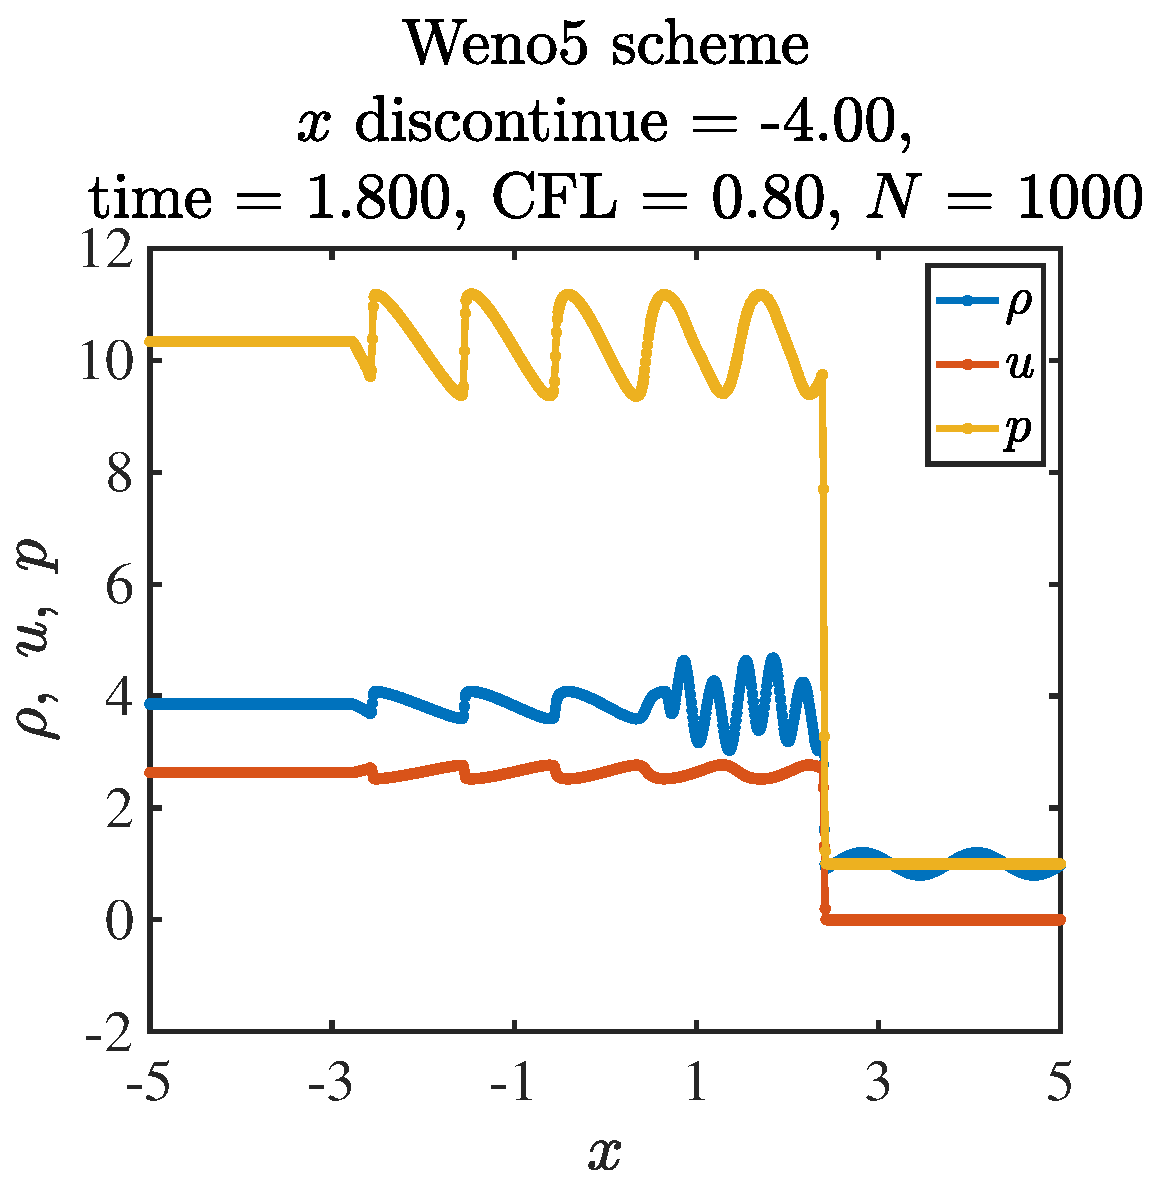
\includegraphics[width=10cm]{4weno5.eps}
	\caption{第四题WENO5格式。}
	\label{fig:4weno5}
\end{figure}


\bibliographystyle{plain}

\phantomsection

\addcontentsline{toc}{section}{参考文献} %向目录中添加条目,以章的名义
\bibliography{homework}

\end{document}
